\chapter{Architettura}\label{cap:architettura}
Nella specifica del problema (rif. \ref{cap:introduzione}) è stato riportato il funzionamento del sistema da realizzare ei relativi componenti neccessari. Per adempire alle richieste della specifica si è deciso di sviluppare l'applicazione dando priorità ai punti fondamentali, dopodichè sono stati trattati gli aspetti secondari come la taratura dei parametri ei meccanismi di richiesta dei servizi. Nella prossima sezione verrà riportata l'architettura del sistema.
\section{Sistema}
\subsection{Composizione Nodi}
Tutta l'applicazione è stata portata avanti considerando la presenza di molteplici nodi richiedenti e fornitori, per rendere possibile una simulazione più reale e complessa. Inizialmente sono state prese delle decisioni inerenti la composizione generale di ogni nodo della nostra rete, in particolare si è deciso di supportate nodi di due tipi:
\begin{description}
\item[wired:] nodo fisso collegato tramite cavo;
\item[wireless:] nodo mobile collegato tramite "etere".
\end{description}
Effettuando tale scelta si sono scatenate un'altra serie di decisioni attinenti l'hardware dei nodi, ovvero l'energia, la memoria ram, il disco e il carico della cpu. Tali componenti sono molto dipendenti dal tipo di collegamento del nodo, in quanto un link di tipo wireless ha bisogno di maggiore calcoli e quindi un utilizzo di energia maggiore.
\begin{figure}[H]
\begin{center}
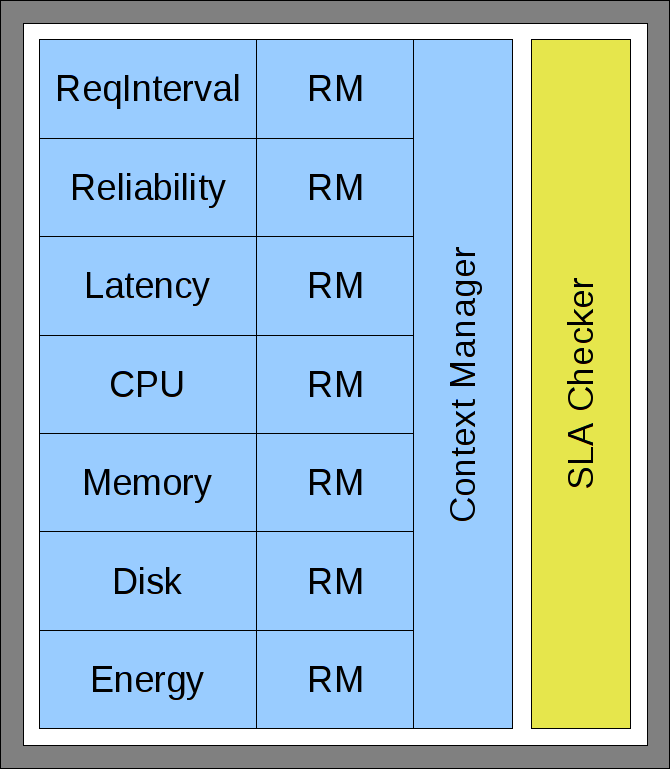
\includegraphics[scale=0.5]{etc/nodo.png}
\caption{Componenti Nodo}
\label{componentinodo}
\end{center}
\end{figure}
Dalla figura \ref{componentinodo} si può notare come è strutturato un singolo nodo, in particolare si può notare come i componenti hardware principali (cpu, memory, disk, energy) siano in stretto contatto con il \var{Context Manager}. Componenti quali: latency, reqInterval e reliability sono a contatto con il \var{Resource Monitor} il quali si occupa appunto di monitorarli. Il componente fondamentale, ovvero lo \var{SLA Checker} (o \var{SC}), si trova in genere a contatto con il \var{CM} e il \var{RM}. Tutte queste parti elencate saranno chiamate d'ora in poi \var{Agenti}, considerando che ci troviamo in ambiente di programmazione ad agenti (ovvero \var{Jade}).
\subsection{Composizione Rete}
La rete che si è deciso di creare è formata da tanti di questi nodi, sia richiedente che fornitore. Nello specifico ogni nodo fornitore si occupa di fornire un servizio generico, il quale viene registrato nelle pagine gialle del sistema. Ogni richiedente, invece, può richiedere il servizio ad uno qualsiasi dei fornitori disponibili. Questa operazione è stata resa possibile per fare in modo che la simulazione si attenesse ad un tipico caso reale. Per quanto riguarda lo \var{SLA Checker} si è progettato il sistema considerando che tale agente dovesse \var{migrare} da un nodo all'altro in base alle condizioni del contesto. Un esempio della rete in questione con 3 nodi può essere visto in figura \ref{rete}. Si può notare che lo \var{SC} si trova solo su uno dei nodi della rete in quanto deve migrare poter migrare fra di loro.
\begin{figure}[H]
\begin{center}
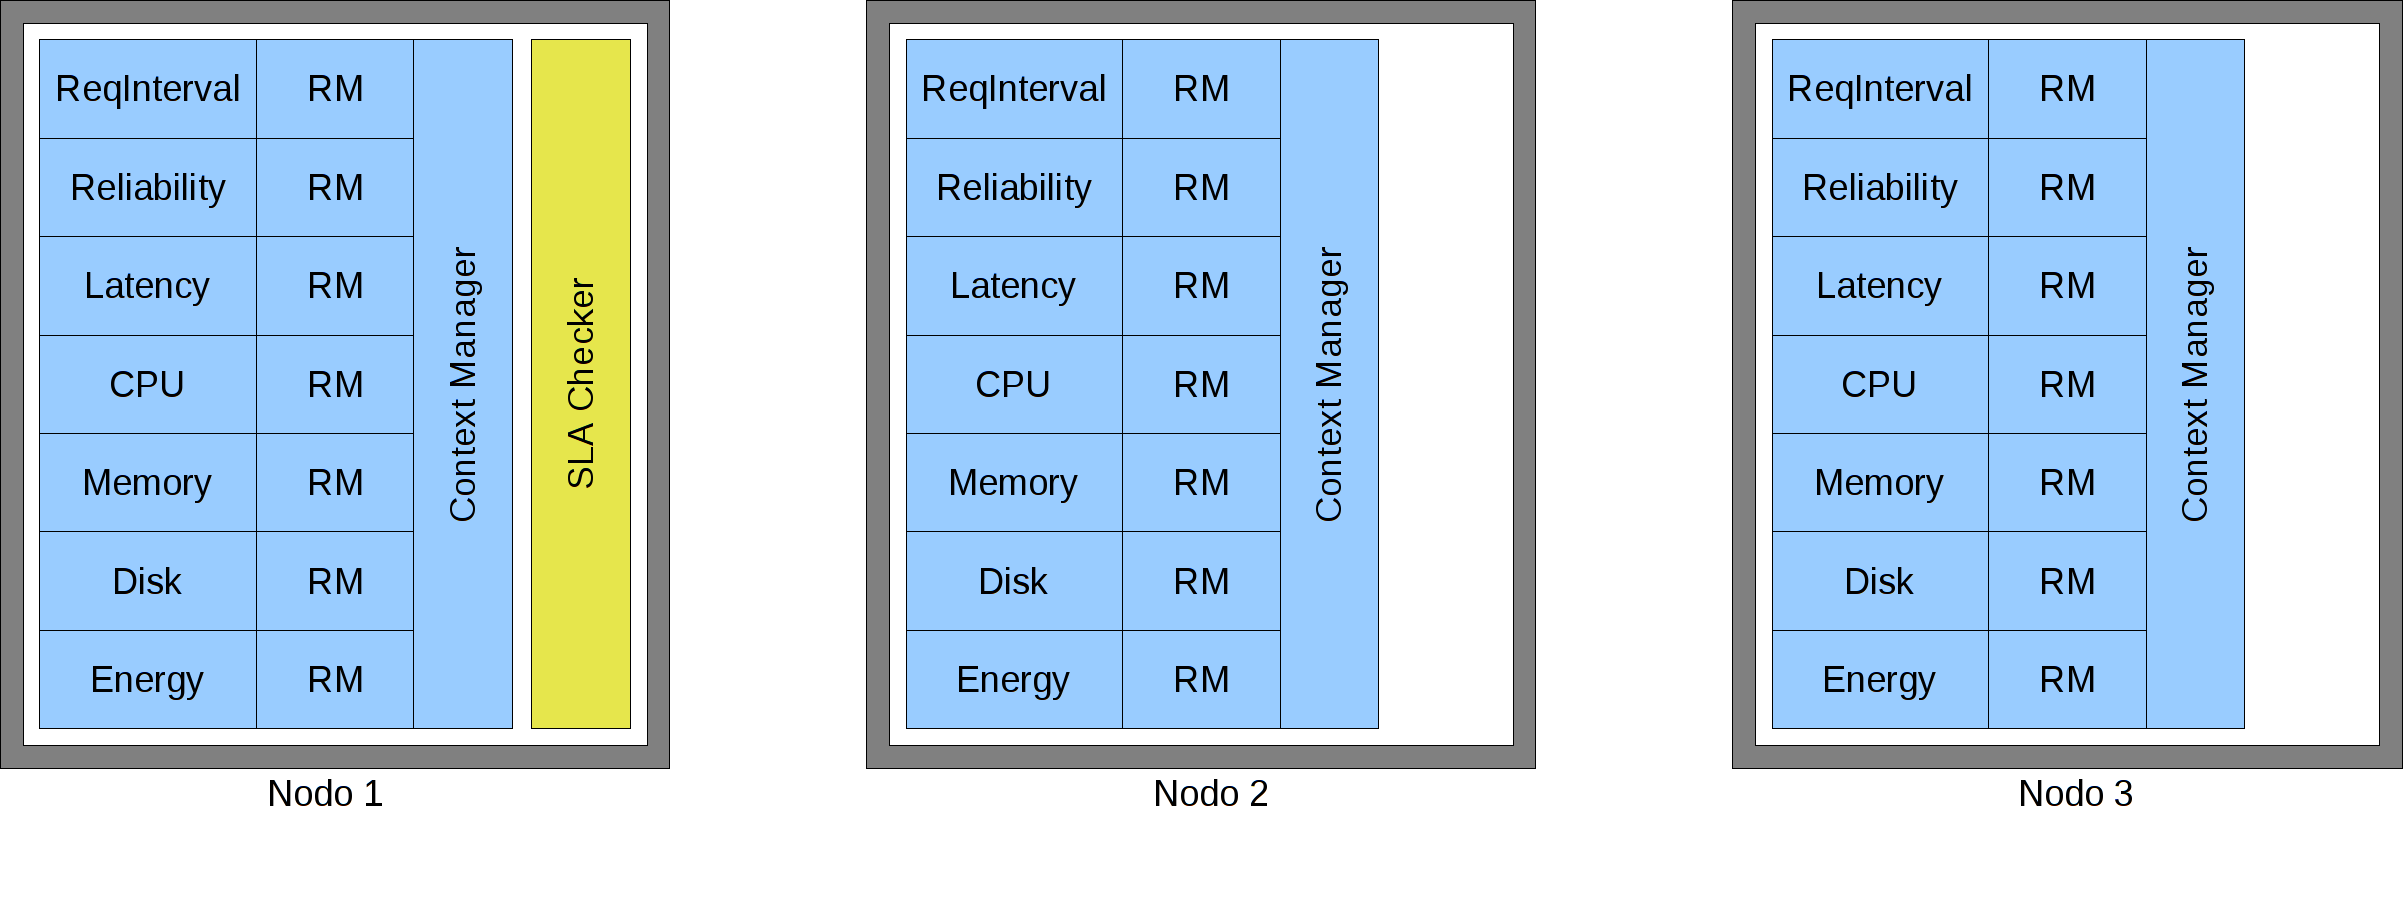
\includegraphics[scale=0.23]{etc/rete.png}
\caption{Esempio di rete con 3 nodi}
\label{rete}
\end{center}
\end{figure}
\section{Funzionamento}
Per spiegare il funzionamento del sistema in questione si è deciso di definire uno scenario d'uso e quindi descrivere il comportamento dei relativi nodi.
\subsection{Scenario d'uso}
Un tipico scenario d'uso potrebbe essere una rete con 3 nodi di cui:
\begin{itemize}
\item 1 nodo fornitore;
\item 2 nodi richiedenti;
\end{itemize}
in particolare ci troviamo in una situazione in cui ognuno dei due nodi richiede un servizio che si attenga al contratto prestabilito con il nodo fornitore. Ogni contratto contiene le seguenti informazioni:
\begin{description}
\item[Publisher:] fornitore del servizio;
\item[Subscriber:] richiedente del servizio;
\item[ReqInterval:] intervallo di tempo tra le richieste del richiedente;
\item[Latency:] tempo impiegato per espletare il servizio;
\item[Reliability:] affidabilità di servizio da parte del fornitore.
\end{description}
Tali informazioni servono per fare in modo che sia il fornitore che il richiedente facciamo il possibile per attenersi ai valori specificati nel contratto.
Su uno dei nodi del sistema è presente lo \var{SLAChecker} che si occupa di controllare la validità di tutti i contratti stipulati. Nel caso in cui le condizioni di un contratto vengono violate da uno dei due nodi allora lo SC informerà immediatamente entrambi i nodi di tale condizione. Tutti i componenti dei nodi sono fortemente dipendenti dalla presenza dello \var{SC}, in quanto comporta un aumento oneroso in termini di calcoli. A causa delle risorse limitate di alcuni nodi (come l'energia) è necessario effettuare un controllo sullo stato attuale dei componenti dei nodi per evitare di sovraccaricarlo. In caso di necessità lo \var{SC} migra su un nodo con condizioni di carico migliori. La selezione del nodo migliore viene fatta utilizzando una specifica politica di selezione (vedi cap. XXX). Un esempio di migrazione può essere visto nelle due figure seguenti, in cui nel primo caso lo SC si trova sul nodo 1, mentre nel secondo caso lo SC è migrato sul nodo 2 a causa di scarsità di risorse sul nodo 1.
\begin{figure}[H]
\begin{center}
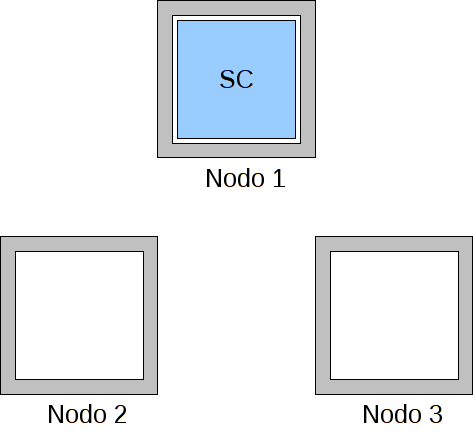
\includegraphics[scale=0.4]{etc/scenario1-1.png}
\caption{Esempio di scenario}
\label{scenario1}
\end{center}
\end{figure}
\begin{figure}[H]
\begin{center}
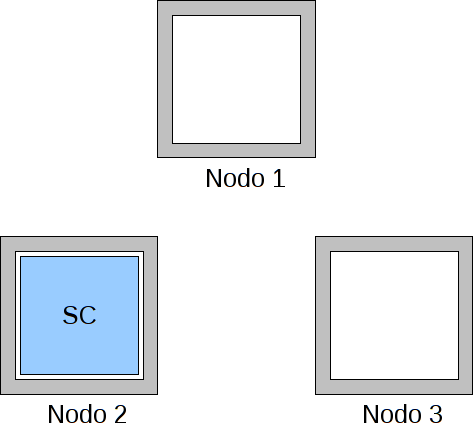
\includegraphics[scale=0.4]{etc/scenario1-2.png}
\caption{Esempio di scenario}
\label{scenario2}
\end{center}
\end{figure}
